\documentclass{beamer}
%
% Choose how your presentation looks.
%
% For more themes, color themes and font themes, see:
% http://deic.uab.es/~iblanes/beamer_gallery/index_by_theme.html
%
\mode<presentation>
{
  \usetheme{default}      % or try Darmstadt, Madrid, Warsaw, ...
  \usecolortheme{default} % or try albatross, beaver, crane, ...
  \usefonttheme{default}  % or try serif, structurebold, ...
  \setbeamertemplate{navigation symbols}{}
  \setbeamertemplate{caption}[numbered]
} 
% CUSTOM
\makeatletter
\newcommand*{\rom}[1]{\expandafter\@slowromancap\romannumeral #1@}
\makeatother

\usepackage[english]{babel}
\usepackage[utf8]{inputenc}
\usepackage[T1]{fontenc}
\usepackage{amsmath}
\usetheme{Antibes}
\usepackage{centernot}
\title[]{Introductory Course: Machine Learning (WWI15B4)}
\subtitle{Classification \rom{2}}
\author{Fabio Ferreira, David Bethge}
\institute{Karlsruhe Institute of Technology}
\date{}
\graphicspath{{figures/04/}}


\expandafter\def\expandafter\insertshorttitle\expandafter{%
   \insertshorttitle\hfill%
   \insertframenumber\,/\,\inserttotalframenumber}
   

\begin{document}
%%%---CUSTOM---
%\bibliographystyle{plain}
%\bibliography{lecture/bibliography.bib}

\begin{frame}
  \titlepage
\end{frame}

\setbeamertemplate{caption}{\raggedright\insertcaption\par}


\section{Classification}
\subsection{Introduction}

\begin{frame}{Example}
\begin{figure}

\includegraphics[width=0.2\textwidth]{cat}
\caption{cat image \emph{x}, shape [100x70x3]} 
\end{figure}



\begin{itemize}
\item parameter vector \emph{W}
\item $f(x,W) \longrightarrow$ 10 values indicating the class scores
\item ideally, the scalar representing 'cat' has highest value
\item W is a parameter vector used in \emph{parametric} function
\end{itemize}
\end{frame}

\begin{frame}{Parametric vs. Non-Parametric}
many definitions, among one is:
\begin{itemize}
\item \textbf{parametric}: model summarizes data by finite set of parameters, e.g. $y_i=\phi_0 + \phi_1x_i + e_i$ 
\item \textbf{non-parametric}: model (user) doesn't make explicit assumptions about the data distribution, e.g. $y_i = f(x_i) + e_i$
\item note: non-parametric methods still require parameters (however, their form isn't defined by the user)
\end{itemize}
\textbf{Task:} Classify the following ML approaches (parametric/non-parametric):
\begin{itemize}
\item decision tree
\item nearest neighbor
\item linear regression
\end{itemize}
\end{frame}


\begin{frame}{Boston House Price dataset}
[The Boston house-price data of Harrison, D. and Rubinfeld, D.L. 'Hedonic
prices and the demand for clean air']
\begin{center}
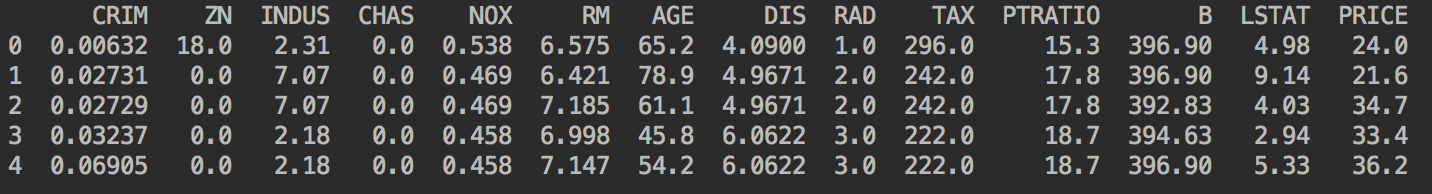
\includegraphics[width=1\textwidth]{boston}\\
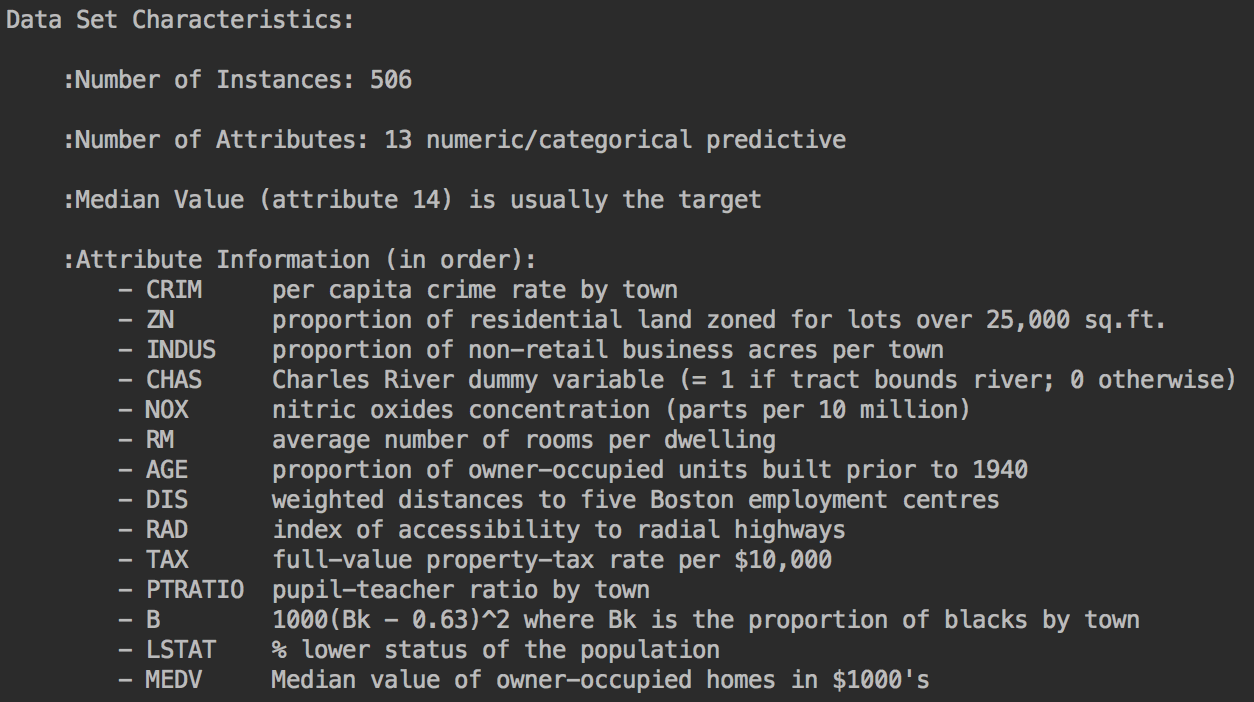
\includegraphics[width=0.7\textwidth, trim=0 9cm 0 0cm]{boston_descr}
\end{center}
\end{frame}

\begin{frame}{Boston House Price dataset}
Boston House Price covariance matrix\\
\begin{center}
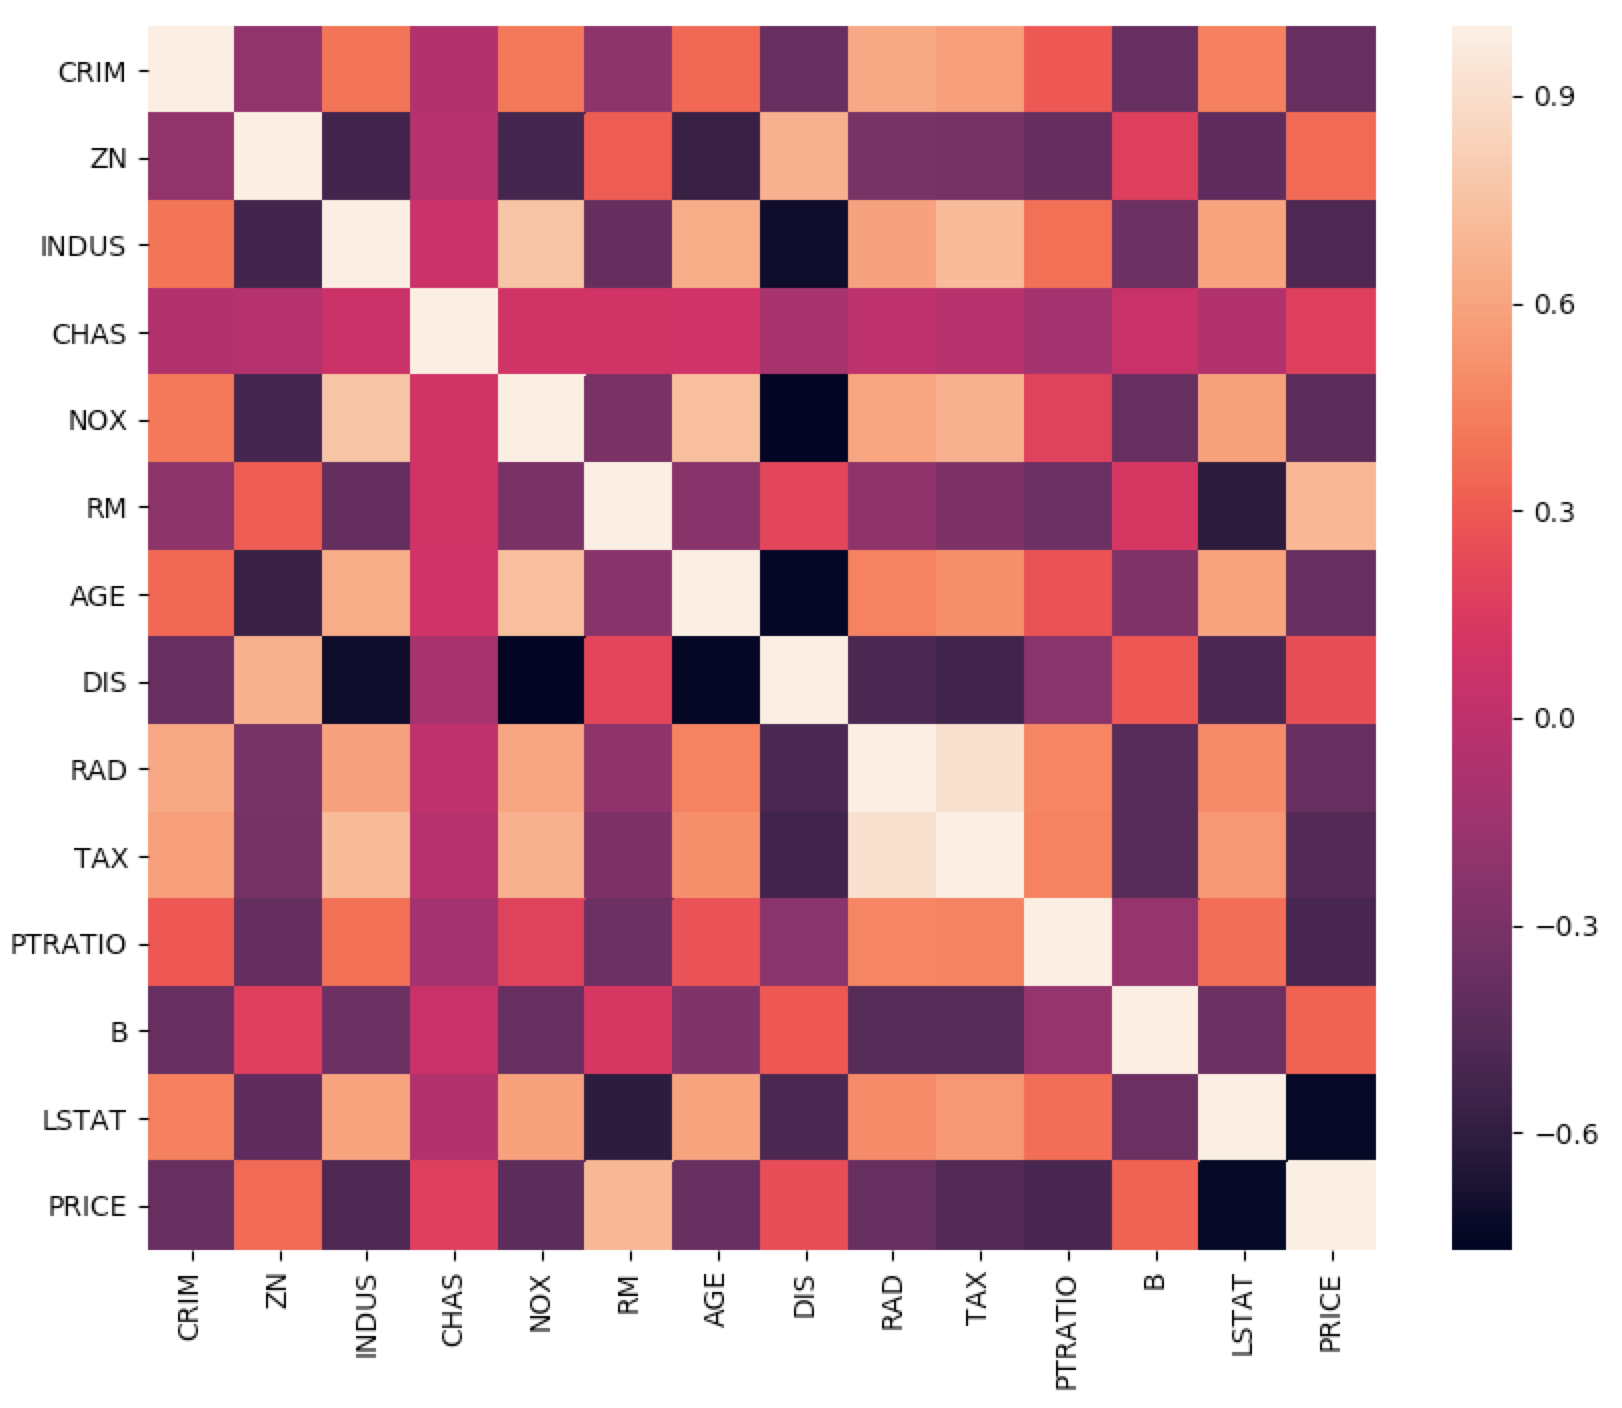
\includegraphics[width=0.65\textwidth]{boston_house_price_correlation}\\
RM: average number of rooms per dwelling
\end{center}
\end{frame}

\begin{frame}{Boston House Price dataset}
Price distribution\\
\begin{center}
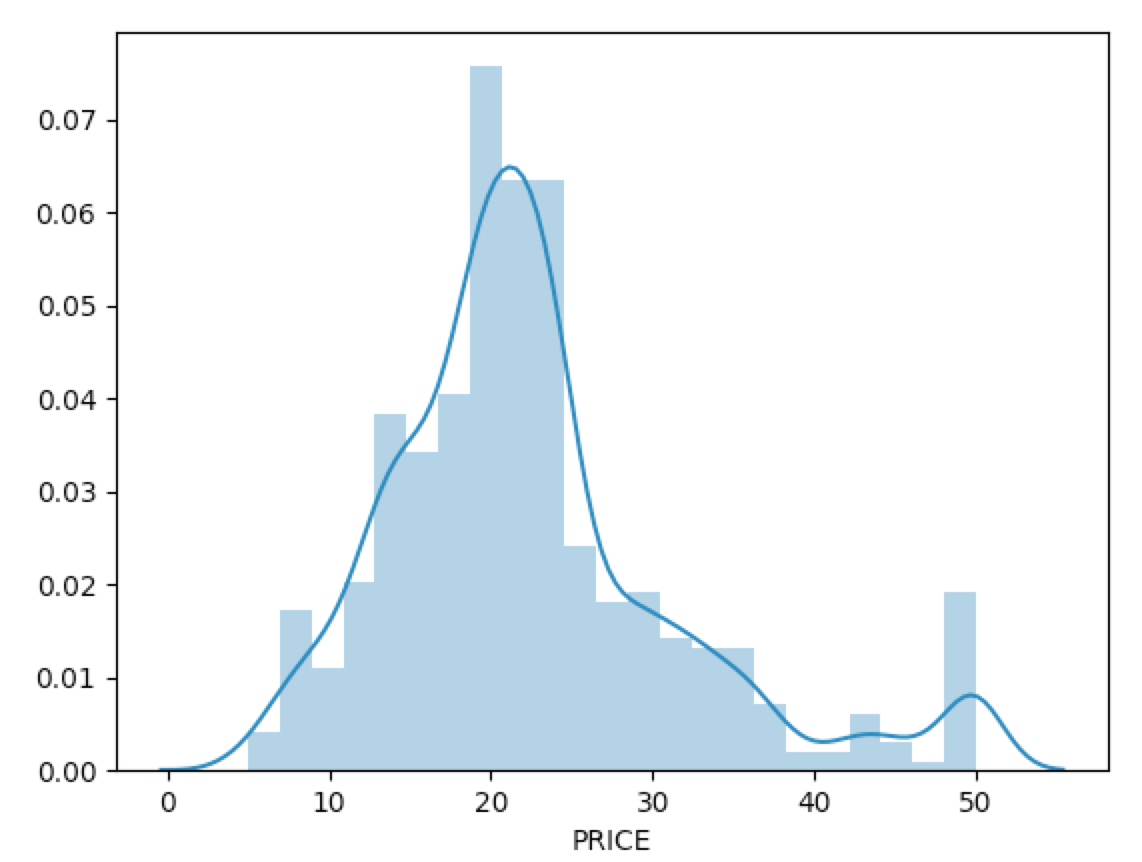
\includegraphics[width=0.80\textwidth]{boston_distr}\\
\end{center}
\end{frame}

\begin{frame}{Boston House Price dataset}
(binary) classification: estimated probability (price > 40) using linear regression (left) and logistic regression (right)\\
\begin{center}
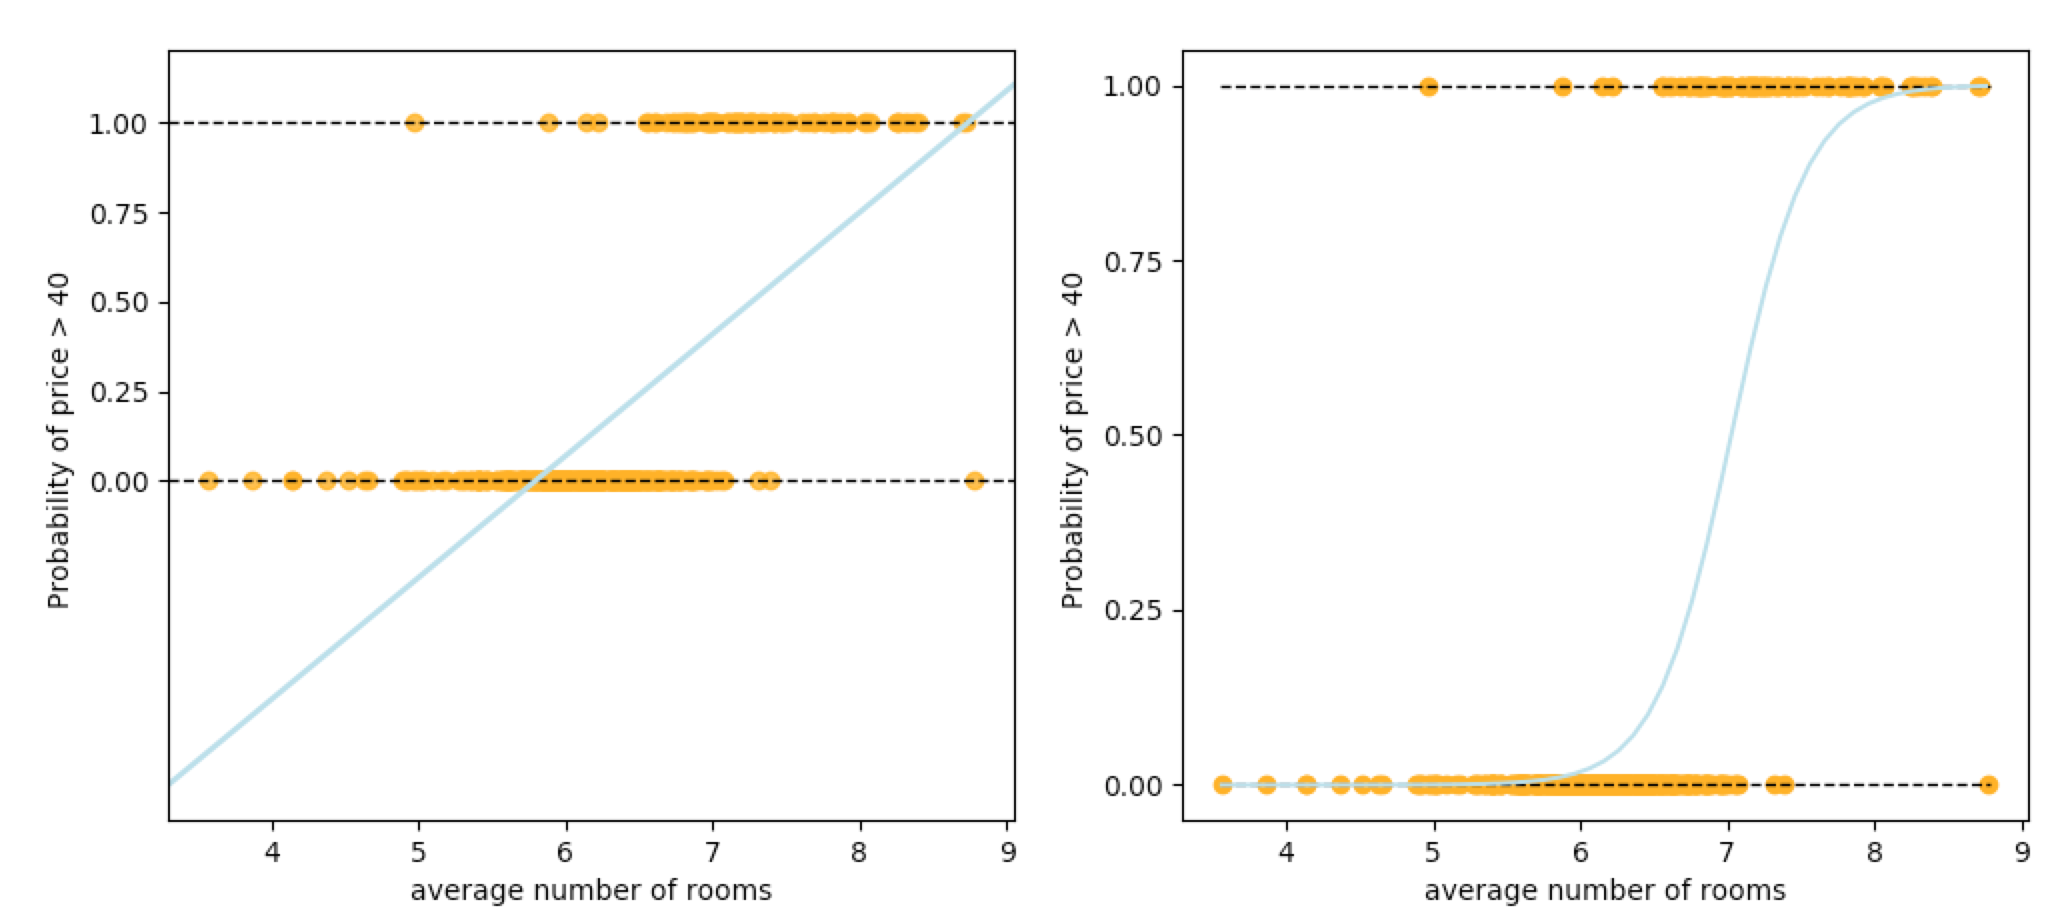
\includegraphics[width=1\textwidth]{log_linear_comparison}\\
\end{center}
\end{frame}

\subsection{Logistic Regression}
\begin{frame}{Logistic Regression}
\begin{itemize}
\item for our linear reg. example we used $p(X) = \beta_0 + \beta_1X$
\item observation: probabilities given by linear reg. can be unreasonable $\rightarrow$ logistic regression
\item terminology recap:
  \begin{itemize}
  	\item X: independent variables, predictors, features
  	\item p(X): dependent variable(s), response 
  \end{itemize}
\item Logistic regression measures the relationship between the categorical dependent variable and one or more independent variables by estimating probabilities using a logistic function
\end{itemize}
\end{frame}

\begin{frame}{Logistic Regression}

\begin{block}{logistic function}
$p(X) = \frac{e^X}{1+e^X} = \frac{1}{1+e^{-X}}$ 
\end{block}
\begin{itemize}
\item which we fit to the model by the use of \emph{maximum likelihood} (later)
\item in our example we had: $p(X) = \frac{1}{1+e^{-\beta_0 - \beta_1X}}$
\item we usually see a transform of the logistic function called \emph{logit}:\\ 
	$log(\frac{p(X)}{1-p(X)}) = \beta_0 + \beta_1X$
\end{itemize}
\end{frame}

\begin{frame}
Mention additional advantages of log. reg.
\end{frame}

\newpage
\bibliographystyle{apalike}
\bibliography{lecture/bibliography.bib}

\end{document}
